%%%%%%%%%%%%%%%%%%%%%%%%%%%%%%%%%%%%%%%%%%%%%%%%%%%%%%%%%%%%%%%%%%%%%%%%%%%%%%%%%%%%%%%%%%%%%%%%%%%%%%%%%%%%%%%%%%%%%%%%%%%%%%%%%%%%%%%%%%%%%%%%%%%%%%%%%%%
% This is just an example/guide for you to refer to when producing your supplementary material for your Frontiers article.                                 %
%%%%%%%%%%%%%%%%%%%%%%%%%%%%%%%%%%%%%%%%%%%%%%%%%%%%%%%%%%%%%%%%%%%%%%%%%%%%%%%%%%%%%%%%%%%%%%%%%%%%%%%%%%%%%%%%%%%%%%%%%%%%%%%%%%%%%%%%%%%%%%%%%%%%%%%%%%%

%%% Version 2.1 Generated 2015/05/22 %%%
%%% You will need to have the following packages installed: datetime, fmtcount, etoolbox, fcprefix, which are normally inlcuded in WinEdt. %%%
%%% In http://www.ctan.org/ you can find the packages and how to install them, if necessary. %%%

\documentclass{frontiers_suppmat} % for all articles

\usepackage{url,hyperref,lineno,microtype}
\usepackage[onehalfspacing]{setspace}
\usepackage{siunitx}

\newcommand{\beq}{\begin{equation}}
\newcommand{\eeq}{\end{equation}}
\newcommand{\beqn}{\begin{equation*}}
\newcommand{\eeqn}{\end{equation*}}
\newcommand{\beqs}{\begin{gather}}
\newcommand{\eeqs}{\end{gather}}
\newcommand{\dd}{\partial}
\newcommand{\vect}[1]{\boldsymbol{#1}}
\newcommand{\vareps}{\varepsilon}
\newcommand{\q}{\boldsymbol{q}}
\newcommand{\vel}{\boldsymbol{u}}
\newcommand{\disp}{\boldsymbol{v}}
\newcommand{\norm}{\boldsymbol{n}}
\newcommand{\ra}{\rightarrow}
\newcommand{\hatz}{\hat{z}}
\newcommand{\hatt}{\hat{t}}
\newcommand{\taurr}{\tau_{rr}}
\newcommand{\taurt}{\tau_{r\theta}}
\newcommand{\tautt}{\tau_{\theta\theta}}
\newcommand{\tauzz}{\tau_{zz}}
\newcommand{\taurz}{\tau_{rz}}
\newcommand{\taurrl}{\tau_{rr,0}}
\newcommand{\taurtl}{\tau_{r\theta,0}}
\newcommand{\tauttl}{\tau_{\theta\theta,0}}
\newcommand{\tauzzl}{\tau_{zz,0}}
\newcommand{\taurzl}{\tau_{rz,0}}
\newcommand{\taurre}{\tau_{rr,1}}
\newcommand{\taurte}{\tau_{r\theta,1}}
\newcommand{\tautte}{\tau_{\theta\theta,1}}
\newcommand{\tauzze}{\tau_{zz,1}}
\newcommand{\taurze}{\tau_{rz,1}}
\newcommand{\err}{e_{rr}}
\newcommand{\ert}{e_{r\theta}}
\newcommand{\ett}{e_{\theta\theta}}
\newcommand{\ezz}{e_{zz}}
\newcommand{\erz}{e_{rz}}
\newcommand{\D}{\Delta}
\newcommand{\Rey}{\mathrm{Re}\xspace}
\newcommand{\Airy}{\mathcal{A}}
\newcommand{\wrt}{w.~r.~t.}
\newcommand{\ie}{i.~e.}


% Leave a blank line between paragraphs in stead of using \\


\def\keyFont{\fontsize{8}{11}\helveticabold }
\def\firstAuthorLast{Diem {et~al.}} %use et al only if is more than 1 author
\def\Authors{Alexandra K. Diem, Neil W. Bressloff, Roxana O. Carare, Matthew MacGregor Sharp and Giles Richardson}
% The Corresponding Author should be marked with an asterisk
% Provide email of the corresponding author
\def\corrAuthor{A.~K.~Diem}
\def\corrEmail{A.K.Diem@soton.ac.uk}


\begin{document}
\onecolumn
\firstpage{1}

\title[Supplementary Material]{{\helveticaitalic{Supplementary Material}}:
\\ \helvetica{Arterial pulsations cannot drive intramural periarterial drainage: Significance for Alzheimer's disease}} %Please insert the title of your article here

\author[\firstAuthorLast ]{\Authors} %This field will be automatically populated
\correspondance{} %This field will be automatically populated

\extraAuth{}% If there are more than 1 corresponding author, comment this line and uncomment the next one.
%\extraAuth{Corresponding Author2: email2@uni2.edu}

\maketitle


\section{Mathematical Analysis of flow through the basement membrane}

This section contains the mathematical derivation of the BM valve model equation. The derivation provided here follows are more analytical approach, while the main text contains a more intuitive derivation.

Recall from the main text the dimensionless governing equations and boundary conditions
\begin{gather}
u_z(r,z,t) = -K(p_z) \frac{\dd p(r,z,t)}{\dd z}\label{eq:uz}\\
u_r(r,z,t) = - \frac{1}{\vareps_L} K(p_z) \frac{\dd p(r,z,t)}{\dd r}\\
\frac{\dd u_z(r,z,t)}{\dd z} + \frac{1}{r} \frac{\dd}{\dd r} \left( ru_r(r,z,t) \right) = 0\label{eq:app_continuity}\\
\frac{\dd R_i(z,t)}{\dd t} = u_r(r,z,t) - u_z(r,z,t) \frac{\dd R_i(z,t)}{\dd z} \qquad \text{on } r = R_i(z,t)\label{eq:ri}\\
\begin{split}
\frac{\dd R_i(z,t)}{\dd t} + \vareps_R \frac{\dd h(z,t)}{\dd t} &=\\
u_r(r,z,t) -& u_z(r,z,t) \left( \frac{\dd R_i(z,t)}{\dd z} + \vareps_R \frac{\dd h(z,t)}{\dd t} \right) \qquad \text{on } r = R_o(z,t).\label{eq:ro}
\end{split}
\end{gather}
Note that here the equations are expressed in terms of velocity $\boldsymbol{u}$ instead of flux $\boldsymbol{q}$. Solving Equation~\ref{eq:app_continuity} for the given boundary condition provides values for the pressure gradient $p_z = \dd p/\dd z$ inside the BM, which is then used to calculate ISF flux through the BM. Performing the variable transformation $(z, r, t) \ra (\hatz, \rho, \hatt)$, with $0 \leq \rho \leq h(z,t)$, such that
\begin{gather*}
z = \hatz\\
r = R_i(z,t) + \vareps_R \rho\\
t = \hatt
\end{gather*}
and thus
\begin{gather*}
\frac{\dd}{\dd z} = \frac{\dd}{\dd \hatz} - \frac{1}{\vareps_R} \frac{\dd R_i(z,t)}{\dd \hatz} \frac{\dd}{\dd \rho}\\
\frac{\dd}{\dd r} = \frac{1}{\vareps_R} \frac{\dd}{\dd \rho}\\
\frac{\dd}{\dd t} = \frac{\dd}{\dd \hatt} - \frac{1}{\vareps_R} \frac{\dd R_i(z,t)}{\dd \hatt} \frac{\dd}{\dd \rho}.
\end{gather*}
Application of the variable transformation to the governing equations (Equation~\ref{eq:uz} to Equation~\ref{eq:app_continuity}) results in
\begin{gather}
\hat{u}_{\hatz}(\hatz,\rho,\hatt) = -K(p_{\hatz} - \frac{1}{\vareps_R} \frac{\dd R_i(z,t)}{\dd \hatz} p_{\rho}) \left( \frac{\dd p(\hatz,\rho,\hatt)}{\dd \hatz} - \frac{1}{\vareps_R} \frac{\dd R_i(z,t)}{\dd \hatz} \frac{\dd p(\hatz,\rho,\hatt)}{\dd \rho} \right)\\
\hat{u}_{\rho}(\hatz,\rho,\hatt) = - \frac{1}{\vareps_R \vareps_L^2} K(p_{\hatz} - \frac{1}{\vareps_R} \frac{\dd R_i(z,t)}{\dd \hatz} p_{\rho}) \frac{\dd p(\hatz,\rho,\hatt)}{\dd \rho}\\
\begin{split}
\frac{\dd \hat{u}_z(\hatz,\rho,\hatt)}{\dd \hatz} - \frac{1}{\vareps_R} \frac{\dd R_i(z,t)}{\dd \hatz} \frac{\dd \hat{u}_z(\hatz,\rho,\hatt)}{\dd \rho} &+\\
\frac{1}{R_i(z,t) + \vareps_R \rho} & \frac{1}{\vareps_R} \frac{\dd}{\dd \rho} \left( \left( R_i(z,t) + \vareps_R \rho \right) \cdot \hat{u}_r(\hatz,\rho,\hatt) \right) = 0,
\end{split}
\end{gather}
while the boundary conditions (Equation~\ref{eq:ri} and Equation~\ref{eq:ro}) become
\begin{gather}
\frac{\dd R_i(z,t)}{\dd \hatt} = \hat{u}_{\rho}(\hatz,\rho,\hatt) - \hat{u}_{\hatz}(\hatz,\rho,\hatt) \frac{\dd R_i(z,t)}{\dd \hatz} \qquad \text{on } \rho = 0\\
\begin{split}
\frac{\dd R_i(z,t)}{\dd \hatt} + \vareps_R \frac{\dd h(z,t)}{\dd \hatt} &=\\
\hat{u}_{\rho}(\hatz,\rho,\hatt) &- \hat{u}_{\hatz}(\hatz,\rho,\hatt) \left( \frac{\dd R_i(z,t)}{\dd \hatz} + \vareps_R \frac{\dd h(z,t)}{\dd \hatz} \right) \qquad \text{on } \rho = h(z,t).
\end{split}
\end{gather}
The next step is to look for a solution in powers of the small parameter $\vareps_R \ll 1$ by writing
\[
p = p_0(\hatz,\hatt) + \vareps_R p_1(\hatz,\rho,\hatt) + \mathcal{O}(\vareps_R^2)
\]
such that the velocity components become
\begin{gather}
\hat{u}_{\hatz}(\hatz,\rho,\hatt) = -K(p_{0\hatz} - \frac{\dd R_i(z,t)}{\dd \hatz} p_{1\rho}) \left( \frac{\dd p_0(\hatz,\hatt)}{\dd \hatz} - \frac{\dd R_i(z,t)}{\dd \hatz} \frac{\dd p_1(\hatz,\rho,\hatt)}{\dd \rho} \right)\label{eq:uz_leading}\\
\hat{u}_{\rho}(\hatz,\rho,\hatt) = - \frac{1}{\vareps_L^2} K(p_{0\hatz} - \frac{1}{\vareps_R} \frac{\dd R_i(z,t)}{\dd \hatz} p_{1\rho}) \frac{\dd p_1(\hatz,\rho,\hatt)}{\dd \rho}\label{eq:ur_leading}.
\end{gather}
Applying this substitution to the governing equations and boundary conditions and letting $\vareps_R \ra 0$ leads to a simplified model in terms of the leading order pressure term $p_0(\hatz,\hatt)$. The governing equations are now Equations~\ref{eq:uz_leading}, \ref{eq:ur_leading} and the continuity equation
\beq
\frac{\dd \hat{u}_{0\hatz}(\hatz,\hatt)}{\dd \hatz} - \frac{\dd R_i(z,t)}{\dd \hatz} \frac{\dd \hat{u}_{1\hatz}(\hatz,\rho,\hatt)}{\dd \rho} + \frac{\dd \hat{u}_{1\rho}(\hatz,\rho,\hatt)}{\dd \rho} + \frac{\hat{u}_{0\rho}(\hatz,\hatt)}{R_i(z,t)} = 0\label{eq:continuity_leading}
\eeq
and the boundary conditions become
\begin{gather}
\frac{\dd R_i(z,t)}{\dd \hatt} = \hat{u}_{0\rho}(\hatz,\hatt) - \hat{u}_{0\hatz}(\hatz,\hatt) \frac{\dd R_i(z,t)}{\dd \hatz} \qquad \text{on } \rho = 0\label{eq:ri_leading}\\
\frac{\dd h(z,t)}{\dd \hatt} = \hat{u}_{1\rho}(\hatz,\rho,\hatt) - \hat{u}_{1\hatz}(\hatz,\rho,\hatt) \frac{\dd h(z,t)}{\dd \hatz} \qquad \text{on } \rho = h(z,t)\label{eq:ro_leading}.
\end{gather} 
To obtain a solution Equation~\ref{eq:continuity_leading} is integrated over the width of the BM \wrt $\rho$
\[
\int_0^{h(z,t)} \left( \frac{\dd \hat{u}_{0\hatz}(\hatz,\hatt)}{\dd \hatz} - \frac{\dd R_i(z,t)}{\dd \hatz} \frac{\dd \hat{u}_{1\hatz}(\hatz,\rho,\hatt)}{\dd \rho} + \frac{\dd \hat{u}_{1\rho}(\hatz,\rho,\hatt)}{\dd \rho} + \frac{\hat{u}_{0\rho}(\hatz,\hatt)}{R_i(z,t)} \right) d\rho = 0
\]
and yields
\beq
h(z,t) \left( \frac{\dd \hat{u}_{0\hatz}(\hatz,\hatt)}{\dd \hatz} + \frac{\hat{u}_{0\rho}(\hatz,\hatt)}{R_i(z,t)} \right) + \left[ \hat{u}_{1\rho}(\hatz,\rho,\hatt) - \frac{\dd R_i(z,t)}{\dd \hatz} \hat{u}_{1\hatz}(\hatz,\rho,\hatt) \right]_0^{h(z,t)} = 0.\label{eq:model_almost}
\eeq
The remaining terms in Equation~\ref{eq:model_almost} can be evaluated using the boundary conditions Equations~\ref{eq:ri_leading} and \ref{eq:ro_leading}. Dropping subscripts the model equation is 
\beq
\frac{\dd}{\dd \hatt} \left( R_i(z,t) \cdot h(z,t) \right) + \frac{\dd}{\dd \hatz} \left( R_i(z,t) \cdot h(z,t) \cdot u(\hatz,\hatt) \right) = 0
\eeq
with 
\[
u = -K(p_{\hatz}) \frac{\dd p(\hatz,\hatt)}{\dd \hatz}
\]

\section{Stress and strain in the artery wall}

All calculations are carried out neglecting body forces such as gravity. Under this assumption stress can only be induced in a solid by applying a force to one of its boundaries. Stress is measured in units of force per area (\SI{}{\newton\per\square\metre}, more commonly denoted as \SI{}{\pascal}). Strain, on the other hand, is a dimensionless quantity that describes the amount of deformation of a solid. Usually, one is interested in strain due to stress, \ie the amount of deformation of a solid due to some force applied to one or more of its boundaries. This relationship between stress and strain is captured in the stress-strain curve, which is unique for every material.

Here, strain is evaluated as the result of stress on the inner boundary of the artery wall. Stress is induced by the pressure pulse running through the artery and is directly proportional to pressure. First, a derivation for obtaining radial stress at any point inside the artery wall is provided. Following this derivation, a fluid-filled annulus representing the BM is introduced inside the artery wall. It is shown that for a sufficiently small BM the fluid-filled annulus can be shrunk to an infinitesimally thin ring. Due to this observation the pressure of ISF inside the BM can be directly obtained from the stress in the artery wall. This pressure serves as an input to the model of the BM derived in Supplementary Section~1.


\subsection{Plane Strain in an Annulus}
\label{sec:planestrain}

Consider an annulus (Supplementary Figure~\ref{fig:annulus}) in the $(r, \theta)$ plane of a cylindrical coordinate system on whose inner boundary ($r = a$) some pressure $P$ is applied. This corresponds to a cross-section of an idealised artery whose centre is aligned with the $z$-axis of the coordinate system. For simplicity $P$ is assumed to be continuous and uniform everywhere on the inner boundary of the annulus. Cauchy's momentum equations \cite{Howell2008}, with displacement $\disp$ independent of $z$ and $t$, are
\begin{gather}
0 = \frac{1}{r} \frac{\dd}{\dd r} \left( r \taurr \right) + \frac{1}{r} \frac{\dd \taurt}{\dd \theta} - \frac{\tautt}{r}\label{eq:cauchy1}\\
0 = \frac{1}{r} \frac{\dd}{\dd r} \left( r \taurt \right) + \frac{1}{r} \frac{\dd \tautt}{\dd \theta} - \frac{\tautt}{r}.\label{eq:cauchy2}
\end{gather}
The components of the stress tensor $\tau$ are
\begin{gather}
\taurr = (\lambda_L + 2\mu_L) \err + \lambda_L \ett \label{eq:taurr}\\
\tautt = \lambda_L \err + (\lambda_L + 2\mu_L) \err \label{eq:tautt}\\
\taurt = 2\mu_L \ert \label{eq:taurt}
\end{gather}
with material specific Lam\'e coefficients $\lambda_L$ and $\mu_L$ and strain tensor $e$ whose components are
\begin{gather}
\err = \frac{\dd v_r}{\dd r}\\
\ett = \frac{1}{r} \left( \frac{\dd v_{\theta}}{\dd \theta} + v_r \right)\\
\ert = \frac{1}{r} \frac{\dd v_r}{\dd \theta} + \frac{\dd v_{\theta}}{\dd r} - \frac{v_{\theta}}{r}.
\end{gather}
As mentioned before pressure is directly proportional to stress and therefore the boundary conditions
\begin{gather}
\taurr = -P \qquad \text{on } r = a\label{eq:boundary_p}\\
\taurr = 0 \qquad \text{on } r = b\label{eq:boundary_b}
\end{gather}
apply. Equation~\ref{eq:boundary_b} is often also referred to as a zero traction boundary condition. Two more boundary conditions are obtained from the fact that the annulus is considered to be radially symmetric and therefore
\begin{gather}
\taurt = 0 \qquad \text{on } r = a\label{eq:boundary_a}\\
\taurt = 0 \qquad \text{on } r = b.\label{eq:boundary_rtb}
\end{gather}

Equation~\ref{eq:cauchy1} and Equation~\ref{eq:cauchy2} and the boundary conditions Equation~\ref{eq:boundary_p}, Equation~\ref{eq:boundary_a} and Equation~\ref{eq:boundary_b} are nondimensionalised using the dimensionless parameters in Supplementary Table~\ref{tab:dimless}
\begin{gather}
0 = \frac{\taurr}{r} + \frac{\dd \taurr}{\dd r} + \frac{\vareps_L}{r} \frac{\dd \taurt}{\dd \theta} - \frac{\tautt}{r}\label{eq:cauchy1_nodim}\\
0 = \frac{\taurt}{r} + \frac{\dd \taurt}{\dd r} + \frac{1}{\vareps_L r} \frac{\dd \tautt}{\dd \theta} - \frac{\tautt}{r}.\label{eq:cauchy2_nodim}\\
\taurr = (1 + 2\vareps_L) \frac{\dd v_r}{\dd r} + \frac{1}{r} \frac{\dd v_{\theta}}{\dd \theta} + \frac{v_r}{r}\label{eq:taurr_nodim}\\
\tautt = \frac{\dd v_r}{\dd r} + (1 + 2\vareps_L) \left( \frac{1}{r} \frac{\dd v_{\theta}}{\dd \theta} + \frac{v_r}{r} \right)\\
\taurt = \frac{1}{r} \frac{\dd v_r}{\dd \theta} + \frac{\dd v_{\theta}}{\dd r} - \frac{v_{\theta}}{r}\label{eq:taurt_nodim}\\
\taurr = -P \qquad \text{on } r = a\\
\taurt = 0 \qquad \text{on } r = a\\
\taurr = \taurt = 0 \qquad \text{on } r = b.
\end{gather}
Expanding the displacement and stress tensor components in terms of the small parameter $\vareps_L$ leads to
\begin{gather*}
v_r = v_{r,0} + \vareps_L v_{r,1} + \mathcal{O}(\vareps_L^2)\\
v_{\theta} = v_{\theta,0} + \vareps_L v_{\theta,1} + \mathcal{O}(\vareps_L^2)\\
\taurr = \taurrl + \vareps_L \taurre + \mathcal{O}(\vareps_L^2)\\
\tautt = \tauttl + \vareps_L \tautte + \mathcal{O}(\vareps_L^2)\\
\taurt = \taurtl + \vareps_L \taurte + \mathcal{O}(\vareps_L^2).\\
\end{gather*}
It is now shown that the leading order terms $\taurrl$ and $\taurtl$ vanish. This follows from the near incompressibility of the arterial wall
\beq
\nabla \cdot \disp = \frac{\dd v_{r,0}}{\dd r} + \frac{v_{r,0}}{r} + \frac{1}{r} \frac{\dd v_{\theta,0}}{\dd \theta} = 0.\label{eq:wall_incompressible}
\eeq
The leading order terms in Equation~\ref{eq:taurr_nodim} to Equation~\ref{eq:taurt_nodim} are\\
\begin{gather}
\taurrl = \frac{\dd v_{r,0}}{\dd r} + \frac{1}{r} \frac{\dd v_{\theta,0}}{\dd \theta} + \frac{v_{r,0}}{r}\label{eq:taurrl}\\
\tauttl = \frac{\dd v_{r,0}}{\dd r} + \frac{1}{r} \frac{\dd v_{\theta,0}}{\dd \theta} + \frac{v_{r,0}}{r}\label{eq:tauttl}\\
\taurtl = \frac{1}{r} \frac{\dd v_{r,0}}{\dd \theta} + \frac{\dd v_{\theta,0}}{\dd r} - \frac{v_{\theta,0}}{r}.
\end{gather}
Both $\taurrl$ and $\taurtl$ are equal to Equation~\ref{eq:wall_incompressible} and therefore indeed vanish. The governing equations Equation~\ref{eq:cauchy1_nodim} and Equation~\ref{eq:cauchy2_nodim} become
\begin{gather}
0 = \frac{\taurre}{r} + \frac{\dd \taurre}{\dd r} + \frac{\vareps_L}{r} \frac{\dd \taurtl}{\dd \theta} + \frac{\vareps_L^2}{r} \frac{\dd \taurte}{\dd \theta} - \frac{\tautte}{r}\label{eq:cauchy1_exp}\\
0 = \frac{\taurtl}{r} + \vareps_L \frac{\taurte}{r} + \frac{\dd \taurtl}{\dd r} + \vareps_L \frac{\dd \taurte}{\dd r} + \frac{1}{\vareps_L r} \frac{\dd \tautte}{\dd \theta} - \frac{\taurtl}{r} - \vareps_L \frac{\taurte}{r}\label{eq:cauchy2_exp}
\end{gather}
and the boundary conditions are
\begin{gather}
\taurre = -P \qquad \text{on } r = a\\
\taurte = 0 \qquad \text{on } r = a\\
\taurre = \taurte = 0 \qquad \text{on } r = b.
\end{gather}
Letting $\vareps_L \ra 0$ and dropping subscripts Equation~\ref{eq:cauchy2_exp} vanishes completely and Equation~\ref{eq:cauchy1_exp} reduces to
\beq
0 = \frac{\taurr}{r} + \frac{d \taurr}{d r} - \frac{\tautt}{r}\label{eq:planestrain}
\eeq
with boundary conditions
\begin{gather}
\taurr = -P \qquad \text{on } r = a\label{eq:plane_bca}\\
\taurr = 0 \qquad \text{on } r = b.\label{eq:plane_bcb}
\end{gather}
The system of Equation~\ref{eq:planestrain} to Equation~\ref{eq:plane_bcb} now only depends on $r$. This makes sense as pressure is applied uniformly across the boundary on $r = a$ and therefore does not vary in the $\theta$-direction. To solve for $\taurr$ an Airy stress function $\Airy(r)$ is used that satisfies the biharmonic equation
\beq
\nabla^4 \Airy(r) = 0.\label{eq:biharmonic}
\eeq
Similar to a stream function in fluid dynamics the Airy stress function is a potential function for the stresses in a solid and is only defined to within a linear function in $r$ \cite{Howell2008}. Again, for readability the notation $\Airy = \mathcal{A}(r)$ is used from now on. To find a solution for $\Airy$ one can begin by defining
\beq
\taurr = \frac{1}{r} \frac{d \Airy}{dr}
\eeq
and from Equation~\ref{eq:planestrain}
\beq
\tautt = \frac{d^2 \Airy}{dr^2}
\eeq
follows. Expanding Equation~\ref{eq:biharmonic} the biharmonic equation for $\Airy$ is
\beq
\frac{1}{r} \frac{d}{dr} \left( r \frac{d}{dr} \left( \frac{1}{r} \frac{d}{dr} \left( r \frac{d\Airy}{dr} \right) \right) \right) = 0,
\eeq
which has a solution of the form
\beq
\Airy = k_1 r^2 + k_2 + k_3 r^2 \log(r) + k_4 \log(r).\label{eq:airy}
\eeq
To solve for the unknown constants $k_1, \ldots, k_4$ the boundary conditions Equation~\ref{eq:plane_bca} and Equation~\ref{eq:plane_bcb} are used. At $r = a$ the stress on the boundary is determined by pressure $P$ such that
\beq
\frac{1}{r} \frac{d\Airy}{dr} = -P \qquad \text{on } r = a.\label{eq:airy_bca}
\eeq 
Equation~\ref{eq:plane_bcb} means that no surface traction is applied on the boundary $r = b$. Surface traction $t(s)$ of arc length $s$ is given by
\beq
t(s) = \frac{d}{ds} \left( \frac{d\Airy}{dr} \right).
\eeq
Integrating \wrt $s$ and applying $t(s) = 0$ gives
\beq
\frac{d\Airy}{dr} = C \qquad \text{on } r = b\label{eq:airy_bcb_c},
\eeq
where $C$ is the constant of integration. Remembering that $\Airy$ is only defined to within a linear function in $r$ one can, without loss of generality, define $C = 0$. Thus, Equation~\ref{eq:airy_bcb_c} becomes
\beq
\frac{d\Airy}{dr} = 0 \qquad \text{on } r = b\label{eq:airy_bcb}.
\eeq
To obtain a condition for $\Airy$ on the boundary $r = b$ rewrite
\beq
\frac{d\Airy}{dr} = \frac{d\Airy}{ds} \vect{e}_t + \frac{d\Airy}{dn} \vect{e}_n,
\eeq
where $\vect{e}_t$ and $\vect{e}_n$ are the unit tangent and outer normal vectors on the boundary. Integrating \wrt $s$ and using Equation~\ref{eq:airy_bcb} yields
\beq
\Airy = 0 \qquad \text{on } r = b.\label{eq:airy_bcb2}
\eeq
Thus far there are three boundary conditions (Equation~\ref{eq:airy_bca}, Equation~\ref{eq:airy_bcb} and Equation~\ref{eq:airy_bcb2}) for the four unknown constants in Equation~\ref{eq:airy}. The fourth condition required to solve Equation~\ref{eq:airy} is called a compatibility condition and is necessary to ensure that the displacement is unique for a certain strain. This condition is not automatically satisfied since there are two stress components $\taurr$ and $\tautt$ for just one displacement component $v_r(r)$. Differentiating $\taurr$ and $\tautt$ and adding them yields the compatibility condition
\beq
\frac{d^3 \Airy}{dr^3} + \frac{1}{r} \frac{d^2 \Airy}{dr^2} - \frac{1}{r^2} \frac{d\Airy}{dr} = 0.
\eeq
which is satisfied only if $k_3 = 0$. Using the boundary conditions to determine the remaining constants results in the solution
\beq
\Airy(r) = \frac{P a^2 b^2}{a^2 - b^2} \cdot \log \left( \frac{r}{b} \right) + \frac{P a^2}{2 (a^2 - b^2)} \left( b^2 - r^2 \right)
\eeq
for a given radial position $r$. The stress components evaluate to
\begin{gather}
\taurr = \frac{P a^2}{b^2 - a^2} \left( 1 - \frac{b^2}{r^2} \right)\label{eq:taurr_airy}\\
\tautt = \frac{P a^2}{b^2 - a^2} \left( 1 + \frac{b^2}{r^2} \right).
\end{gather}
The Airy stress function approach provides a solution for a material with a linear stress-strain relation.


\subsection{Validation of the Plane Strain Model}

The plane strain model for calculating the stresses inside an artery makes a number of simplifying assumptions:
\begin{enumerate}
\item Stress is calculated without regard for the longitudinal $z$-direction.
\item The artery wall is a linear elastic material.
\item Pressure inside the artery is uniform across the lumen area.
\end{enumerate}
The validity of these assumptions shall be addressed in this section before proceeding with an adaptation of the plane strain model to obtain ISF pressure inside the BM.

The first assumption arises from the fact that blood vessels are longitudinally tethered, \ie both ends of the arterial tree are attached to the heart, which limits the amount of stretch they can undergo along the $z$-direction. This assumption has been used in the literature and the same equations have successfully been used to accurately describe blood flow dynamics by others \cite{Olufsen2000,Kolachalama2007,Devault2008,Cousins2014}. To evaluate the second assumption one has to recognise that the artery wall actually is a viscoelastic material. This means that there is a time delay between an increase in blood pressure (\ie increased radial stress on the artery wall) and the corresponding increase in vessel diameter. This effect cannot accurately be captured by a purely elastic material. However, \cite{Tardy1991} showed that this time lag is mainly an experimental artefact and have developed a model to correct experimental measurements for this artefact. No other publication could be found to investigate this hypothesis, but results from other blood flow simulation studies show that this simple model appears to suffice to accurately model blood flow dynamics.

To confirm the second and address the third assumption a simple model was set up in the finite element multiphysics modelling software COMSOL 5.1. The geometry is a 2D axisymmetric tube of length $L_0$ with radius $R_0$ surrounded by a wall of thickness $h_0$. Flow inside the tube is governed by the Navier-Stokes equations for laminar flow
\begin{gather}
\rho (\vel \cdot \nabla) \vel = \nabla \cdot \left( -p \boldsymbol{I} + \mu \left( \nabla \vel + (\nabla \vel)^T \right) \right) + \boldsymbol{F}_s\\
\rho \nabla \cdot \vel = 0
\end{gather}
with $\boldsymbol{I}$ identity matrix and $\boldsymbol{F}_s$ some external body force. The dynamics of the wall are governed by either the equations for linear elasticity or hyperelasticity. In both cases the stress relates to $\boldsymbol{F}_s$ via
\beq
-\nabla \sigma = \boldsymbol{F}_s \nu_s\\
\eeq
with $\sigma$ stress tensor and $\nu_s$ Poisson's ratio. In the case of the linear elastic model stress is governed by Hooke's law
\begin{gather}
\sigma = \sum_i \sum_j C_{ij} \vareps_{\text{el},ji}\\
\vareps_{\text{el}} = \frac{1}{2} \left( (\nabla \disp)^T + \nabla \disp + (\nabla \disp)^T \nabla \disp \right) 
\end{gather}
with $C$ elasticity tensor and $\vareps_{\text{el}}$ elastic strain tensor. In the case of nonlinear elasticity stress is governed by a Neo-Hookean material model, which has been shown to provide a good fit for the mechanical response of arterial elastin \cite{Holzapfel1998,Gundiah2007}, where stress is given as
\beq
\sigma = J^{-1} \boldsymbol{F}_s \boldsymbol{S}_s \boldsymbol{F}_s^T
\eeq
with $J = \det(\boldsymbol{F}_s)$ and $\boldsymbol{S}_s = \dd W_s / \dd \vareps_{el}$ second Piola-Kirchoff stress. For a nearly incompressible neo-Hookean material the strain energy density function is
\beq
W_s = W_{\text{iso}} + W_{\text{vol}} = \frac{1}{2} \mu_s (\bar{I}_1 - 3) + \frac{1}{2} K_s (J_{\text{el}} - 1)^2,
\eeq
where $\mu_s$ initial shear modulus, $\bar{I}_1$ first principal invariant of the symmetric right Cauchy-Green tensor, $K_s$ initial bulk modulus and $J_{\text{el}}$. The boundary between the lumen and artery wall implements a two-way coupling between the two domains: In the fluid domain pressure is determined by the normal stress on the wall
\beq
\sigma \cdot \norm = \left( -p \boldsymbol{I} + \mu \left( \nabla \vel + (\nabla \vel)^T \right) \right) \cdot \norm,
\eeq
while the rate of displacement of the artery wall is determined by the fluid velocity
\beq
\frac{\dd \disp}{\dd t} = \vel.
\eeq
Because the artery is tethered displacement of the artery wall is restricted to the $z$-direction at open ends
\beq
\disp \cdot \norm = 0.
\eeq
At the fluid inlet a velocity is applied, while at the outlet pressure is applied. The parameter values used for the simulations are listed in Supplementary Table~\ref{tab:airy_sim}.

The results of this simulation are shown in Supplementary Figure~\ref{fig:linear_hyperelastic}. There is good agreement between the hyperelastic and linear elastic material while the Airy stress function overestimates hoop stress ($\tau_{\theta\theta}$) at the higher end of the pressure range. This is acceptable as an overestimation of stress would lead to an overestimation of ISF pressure inside the BM. If ISF pressure inside the BM is too small to drive significant flow when stress is estimated using the Airy stress function then it will also be too small when using a hyperelastic numerical simulation. Furthermore, only radial stress is required for the calculation of ISF pressure and the overall agreement between the Airy stress function and the simulation results is found to be suitably good for radial stress. Therefore the Airy stress function calculation was used for the remainder of this thesis. 


\subsection{Plane Strain in an Artery Cross-Section with BM}
\label{sec:bm_stress}

The Airy stress function derived in Section~\ref{sec:planestrain} can also be used to determine the pressure of ISF in the BM. For simplicity the BM shall be treated as a thin fluid-filled empty space. This approximation is considered valid for the fluid part of a porous medium if the fluid-filled space is small enough. The BM is only approximately \SI{150}{\nano\metre} in thickness, which is roughly three orders of magnitude smaller than the thickness of the artery wall of the MCA and therefore, the approximation is considered valid. Two independent Airy stress functions $\Airy_1(r)$ and $\Airy_2(r)$ are thus used to describe the artery wall parts surrounding the BM (Supplementary Figure~\ref{fig:twoannuli}). Following the analysis in Section~\ref{sec:planestrain} these are
\begin{gather}
\Airy_1 = k_1 r^2 + k_2 + k_3 \log(r)\\
\Airy_2 = k_4 r^2 + k_5 + k_6 \log(r)
\end{gather}
and as before the boundary conditions are
\begin{gather}
\frac{1}{r} \frac{d \Airy_1}{dr} = -P \qquad \text{on } r = a_1\\
\Airy_2 = \frac{d \Airy_2}{dr} = 0 \qquad \text{on } r = b_2.
\end{gather}
The pressure of ISF $P_{BM}$ is required to be continuous and uniform and therefore
\beq
\frac{d \Airy_1}{dr} = \frac{d \Airy_2}{dr} \qquad \text{on } r = b_1, a_2
\eeq
applies. 

The claim that, given a sufficiently thin BM, a single Airy stress function can be used to model the artery wall like in Section~\ref{sec:planestrain} and the ISF pressure can then be directly obtained from the stress in the wall at the location of the BM shall be proven here. Because ISF is an incompressible fluid its area $A_f$ has to remain constant
\beq
A_f = \pi \left( \left( a_2 + v_r(a_2) \right)^2 - \left( b_1 + v_r(b_1) \right)^2 \right) = const.
\eeq
Eliminating $\pi$ and the small square terms in $v_r$ yields
\beq
2a_2 v_r(a_2) - 2b_1 v_r(b_1) = b_1^2 - a_2^2.
\eeq
As the fluid part of the BM is considered to be very thin one can take the limit
\beq
\lim_{b_1 \ra a_2} 2a_2 v_r^+(a_2) - 2b_1 v_r^-(b_1) = b_1^2 - a_2^2.
\eeq
and confirm
\beq
v_r^+(a_2) = v_r^-(b_1).
\eeq
Therefore $\Airy_1$ and $\Airy_2$ must be continuous across the BM such that
\beq
\Airy_1 = \Airy_2 \qquad \text{on } r = b_1, a_2.
\eeq
Therefore the claim is proven and a single Airy stress function $\Airy = \Airy_1 + \Airy_2$ can be used to describe the artery wall. The ISF pressure can then be found by evaluating $\taurr$ (Equation~\ref{eq:taurr_airy}) at $r = b_1$
\beq\label{eq:bm_pressure}
P_{\text{BM}} = - \frac{P a_1^2}{b_2^2 - a_1^2} \left( 1 - \frac{b_2^2}{b_1^2} \right).
\eeq


\bibliographystyle{frontiersinSCNS_ENG_HUMS} % for Science, Engineering and Humanities and Social Sciences articles, for Humanities and Social Sciences articles please include page numbers in the in-text citations
%\bibliographystyle{frontiersinHLTH&FPHY} % for Health and Physics articles
\begin{thebibliography}{10}
\bibitem{Howell2008}
Howell~P, Kozyreff~G and Ockendon~J (2008) {\em Applied Solid Mechanics.} Cambridge University Press, Cambridge, UK.

\bibitem{Olufsen2000}
Olufsen~MS et~al. (2000) Numerical Simulation and Experimental Validation of Blood Flow in Arteries with Structured-Tree Outflow Conditions. {\em Ann.~Biomed.~Eng.} 28(11):1281--1299.

\bibitem{Kolachalama2007}
Kolachalama~V, Bressloff~NW, Nair~PB, Shearman~CP (2007) Predictive Haemodynamics in a One-Dimensional Carotid Artery Bifurcation. Part I: Application to Stent Design. {\em IEEE~Trans.~Biomed.~Eng.} 54(5):802--812.

\bibitem{Cousins2014}
Cousins~W, Gremaud~PA (2014) Impedance boundary conditions for general transient hemodynamics. {\em Int.~J.~Numer.~Method~Biomed.~Eng.}

\bibitem{Devault2008}
Devault~K and Gremaud~A (2008) Blood Flow in the Circle of Willis: Modeling and Calibration. {\em Multiscale~Model.~Simul.} 7(2):888--909.

\bibitem{Tardy1991}
Tardy~Y, Meister~JJ, Perret~F, Brunner~HR and Arditi~M (1991) Non-invasive estimate of the mechanical properties of peripheral arteries from ultrasonic and photoplethysmographic measurements. {\em Clin.~Phys.~Physiol.~Meas.} 12(1):39--54.

\bibitem{Holzapfel1998}
Holzapfel~GA and Weizsacker~HW (1998) Biomechanical behaviour of the arterial wall and its numerical characterization. {\em Comput.~Biol.~Med.} 28(4):377--392.

\bibitem{Gundiah2007}
Gundiah~N, Ratcliffe~MB and Pruitt~LA (2007) Determination of strain energy function for arterial elastin: Experiments using histology and mechanical tests. {\em J.~Biomech.} 40(3):586--594.  
\end{thebibliography}


\begin{table}[h]
\textbf{\refstepcounter{table}\label{tab:dimless} Supplementary Table \arabic{table}.}{ Dimensionless variables and parameters used to nondimensionalise the equations of the stress tensor components of an inflated annulus (Equation~\ref{eq:taurr}, Equation~\ref{eq:tautt} and Equation~\ref{eq:taurt}). }

\processtable{ }
{\begin{tabular}{cc}\toprule
Parameter & Physical meaning \\\midrule
$L$         & length\\
$R$         & radius\\
$V$         & tangential displacement\\
$\lambda_L$ & first Lam\'e coefficient\\
$\mu_L$ & second Lam\'e coefficient\\
$\vareps_L = R/L \ll 1$ & radius-to-length ratio\\
\midrule
Variable       & \\
\midrule
$r \sim R = \vareps_L L$ & radius\\
$v_{r} \sim \vareps_L V$ & radial displacement\\
$v_{\theta} \sim V$ & tangential displacement\\
$\taurr \sim \lambda_L V/L$ & radial stress\\
$\tautt \sim \lambda_L V/L$ & hoop stress\\
$\taurt \sim \mu_L V/L$ & \\
$P \sim \lambda_L V/L$ & blood pressure\\\botrule
\end{tabular}}{}
\end{table}

\begin{table}[h]
\textbf{\refstepcounter{table}\label{tab:airy_sim} Supplementary Table \arabic{table}.}{ Parameters used in the linear and hyperelastic FE simulation of an artery. }

\processtable{ }
{\begin{tabular}{ccc}\toprule
Parameter & Value & Physical meaning \\\midrule
$R$ & \SI{0.134}{\centi\metre} & vessel radius\\
$L$ & \SI{1.2}{\centi\metre} & vessel length\\
$h$ & $R/4$ & wall thickness\\
$u_\text{in}$ & \SI{0.6}{\centi\metre\per\second} & inlet velocity\\
$p_\text{out}$ & 80 / 100 / \SI{120}{\mmHg} & outlet pressure\\
$\mu$ & \SI{4.88e-3}{\pascal\second} & dynamic viscosity of blood\\
$\rho$ & \SI{1.06}{\gram\per\cubic\metre} & blood density\\
$\rho_s$ & \SI{0.9}{\gram\per\cubic\metre} & artery wall density\\
\midrule
\multicolumn{3}{l}{Linear elastic material properties}\\
\midrule
$E$ & \SI{7.37e5}{Pa} & Young's modulus\\
$\nu_s$ & 0.495 & Poisson's ratio\\
\midrule
\multicolumn{3}{l}{Hyperelastic material properties}\\
\midrule
$\mu_s$ & $E / (2 (1 + \nu))$ & initial shear modulus\\
$K_s$ & $E / (3 (1 - 2\nu))$ & initial bulk modulus\\\botrule
\end{tabular}}{}
\end{table}

\begin{figure}
\begin{center}
\includegraphics[width=15cm]{figures/annulus.pdf}% This is a *.jpg file
\end{center}
\textbf{\refstepcounter{figure}\label{fig:annulus} Supplementary Figure \arabic{figure}.}{ Schematic representation of a linear elastic annulus in the $(r, \theta)$ plane inflated by an internal pressure $P$. }
\end{figure}

\begin{figure}
\begin{center}
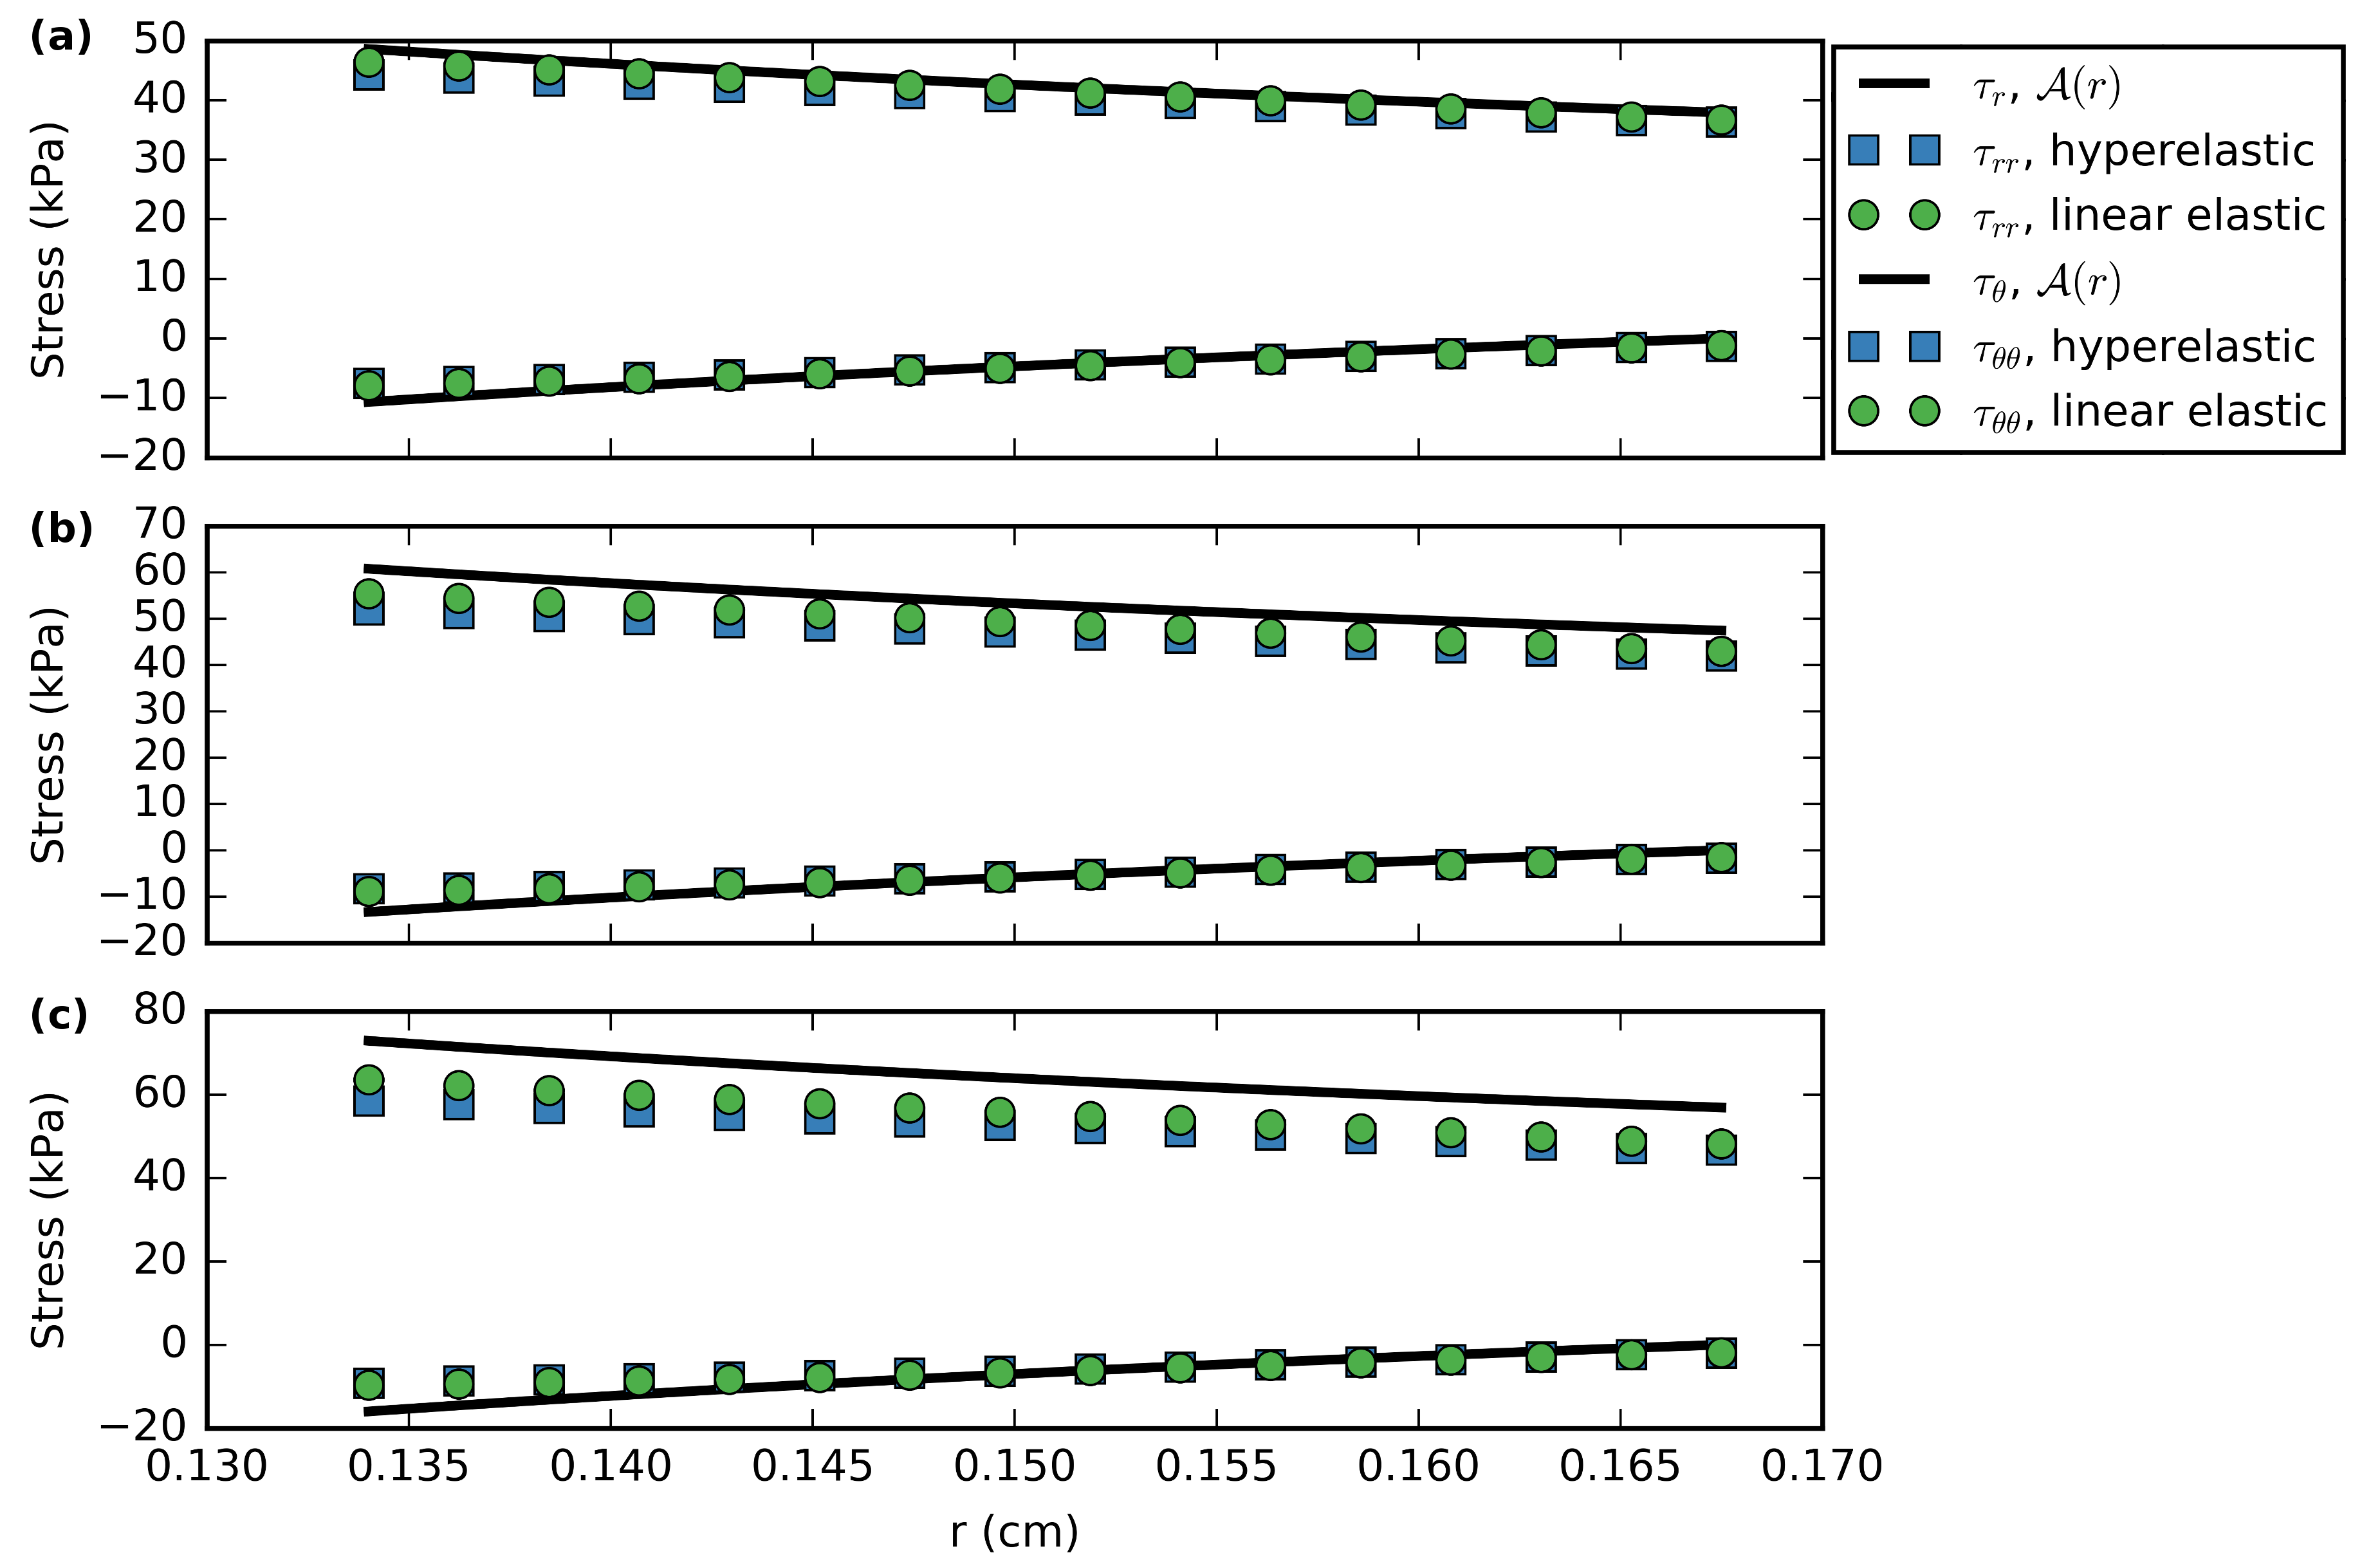
\includegraphics[width=15cm]{figures/linear_hyperelastic.png}% This is a *.jpg file
\end{center}
\textbf{\refstepcounter{figure}\label{fig:linear_hyperelastic} Supplementary Figure \arabic{figure}.}{ Comparison of radial and hoop stresses in an artery wall using the Airy stress function (black line) or an FE simulation with linear (green circles) or hyperelastic (blue squares) material at various blood pressures. (a) $p = \SI{80}{\mmHg}$, (b) $p = \SI{100}{\mmHg}$, (c) $p = \SI{120}{\mmHg}$. }
\end{figure}

\begin{figure}
\begin{center}
\includegraphics[width=15cm]{figures/twoannuli.pdf}% This is a *.jpg file
\end{center}
\textbf{\refstepcounter{figure}\label{fig:twoannuli} Supplementary Figure \arabic{figure}.}{ Schematic representation of the elastic model of an artery cross-section with BM inflated by an internal pressure $P$. For simplicity the BM is approximated by a fluid-filled space at some radial position $r$. The artery wall is then split into two separate parts, which are described by two independent Airy stress functions $\Airy_1$ and $\Airy_2$. }
\end{figure}

\end{document}
